\documentclass[article, nojss]{jss}

%%%%%%%%%%%%%%%%%%%%%%%%%%%%%%
%% declarations for jss.cls %%%%%%%%%%%%%%%%%%%%%%%%%%%%%%%%%%%%%%%%%%
%%%%%%%%%%%%%%%%%%%%%%%%%%%%%%

%% almost as usual
\author{Hannes Matuschek\\University of Potsdam, Germany}
\title{\pkg{StochBB}: A Software Framework and Application for Analyzing Networks of Random Variables}

%% for pretty printing and a nice hypersummary also set:
\Plainauthor{Hannes Matuschek} %% comma-separated
\Plaintitle{StochBB: A Software Framework and Application for Analyzing Networks of Random Variables} %% without formatting
\Shorttitle{\pkg{StochBB}: Analyzing Networks of Random Variables} %% a short title (if necessary)

%% an abstract and keywords
\Abstract{
  \pkg{StochBB} is a sofware framework and a graphical user interface program that allows of an efficient
analysis of complex systems of dependent random variables. For example, such networks are 
frequently used to describe cognitive processes and are usually analyzed by means of Monte Carlo
type stochastic simulations. Although very flexible, the stochastic simulation approach requires a
large number of samples to be drawn, for obtaining reliable statistics of the response variable of
interest. In contrast to stochastic simulation, \pkg{StochBB} derives the marginal distributions of
dependent random variables analytically and resorts to numerical solutions whenever the analytic
approach fails. To achieve this,  \pkg{StochBB} implements a rudimentary computer algebra system
for systems of dependent random variables. As an example, I study the properties of a simple 
response-latency model.

}

\Keywords{random variables, computer algebra system, stochastic simulation, \proglang{C++}, \proglang{Python}, \proglang{R}}
\Plainkeywords{random variables, computer algebra system, stochastic simulation, C++, Python, R} %% without formatting
%% at least one keyword must be supplied

%% publication information
%% NOTE: Typically, this can be left commented and will be filled out by the technical editor
%% \Volume{50}
%% \Issue{9}
%% \Month{June}
%% \Year{2012}
%% \Submitdate{2012-06-04}
%% \Acceptdate{2012-06-04}

%% The address of (at least) one author should be given
%% in the following format:
\Address{
  Hannes Matuschek\\
  Department of Mathematics\\
  Focus area \emph{Dynamics of Complex Systems}\\
  University of Potsdam\\
  Karl-Liebknecht-Strasse 24-25\\
  D-14476 Potsdam, Germany\\
  E-mail: \email{hannes.matuschek@uni-potsdam.de}\\
}
%% It is also possible to add a telephone and fax number
%% before the e-mail in the following format:
%% Telephone: +43/512/507-7103
%% Fax: +43/512/507-2851

%% for those who use Sweave please include the following line (with % symbols):
%% need no \usepackage{Sweave.sty}

%% end of declarations %%%%%%%%%%%%%%%%%%%%%%%%%%%%%%%%%%%%%%%%%%%%%%%

\usepackage{listings}
\usepackage{amsmath}
\usepackage{color}
\usepackage{graphicx}
\usepackage{subcaption}
\usepackage{editorial}

\begin{document}

\section{Introduction} \label{sec:intro}
Frequently, complex systems are described in terms of stochastic processes, as the
underlying deterministic process is too complex to be modeled exactly or as the
process is indeed random. It is not always the random process itself that is of 
interest, but a derived quantity. For example, the distribution of waiting times until the
process reaches a certain state. In the field of cognitive psychology, random processes are frequently used to
describe each processing stage in a chain of stages that leads to a response. The state of
each random process itself is usually not measurable but the total response time of all processing 
stages involved. Although each processing stage may be modeled as a random process, the waiting-time
of a single stage is just a sample of a random variable%
\footnote{This requires that the random process is \emph{reset} for each sample. This is usually 
the case if the waiting time of the processing stage is determined by the time a random process
starting at a specified state reaches a certain end state. Then, the waiting times of the processing
stage are independent samples from a simple random variable with some distribution.}%
and the complete system is therefore a 
system of dependent random variables \cite[e.g., the EZ-Reader model,][]{Reichle2003}.

\pkg{StochBB} is able to describe and analyze complex systems of dependent random variables
by combining simple ones (representing single stages with a known waiting-time distribution) to
a complex system. For example, consider the following independent random variables
\begin{equation}
  X_1 \sim \Gamma(10, 100)\,, X_2 \sim \Gamma(20, 50)\text{ and } X_3 \sim \text{Exp}(0.01)\,,\nonumber
\end{equation}
which are described completely by their distribution. This means that the time, the
processing stage $X_1$ needs to complete is gamma-distributed with shape $k=10$ and scale
$\theta=100$. Analogously, the stages $X_2$ and $X_3$ are defined by their own waiting-time 
distribution.

From these basic building blocks, a more complex system can be assembled by
combining them. Using the example above, one may define a new processing stage that is a chain of
the stages $X_1,\dots,X_3$. This simple chain then describes the successive
processing of information entering the first stage described by $X_1$.
Once the first processing stage finishes, its result gets forwarded to the second stage described
by $X_2$ and finally to the last stage described by $X_3$. The waiting time of the
complete chain is again a random variable that is the sum of all random variables,
or expressed mathematically
\begin{equation}
 Y = X_1 + X_2 + X_3\,. \nonumber
\end{equation}

\pkg{SochBB} determines the probability density function (PDF) or cumulative probability function
(CDF) of the waiting-time distribution of the process $Y$ analytically (as far as
possible) or resorts to a numeric method if the analytic approach fails 
\cite[see][for examples of numerical approximations outperforming the stochastic simulation approach]{Thomas2012, Thomas2013}.
Moreover it provides an efficient and correct sampler for the system of random variables.

\marked{TODO: Briefly outline the paper here.}

\section{Representation and reductions of random variables}
Continuing the example above, please note that the sum of random variables commutes. Hence the
random variable $Y$ remains the same if defined as $Y = X_1 + X_3 + X_2$ instead of 
$Y = X_1 + X_2 + X_3$. Moreover, the 
distribution of the sum of $X_1$ and $X_3$ can be determined analytically as 
$X' = (X_1+X_3)\sim\Gamma(11,100)$. Hence the random variable $Y$ can now be expressed as 
$Y = X_2 + X'$, and only a single numeric convolution is necessary to obtain the PDF of the
random variable $Y$. \pkg{SochBB} implements several reductions, exploiting mathematical
identities of random variables and their distributions. To this end, it allows to obtain their PDFs and 
CDFs efficiently. In this section, all basic building blocks that are currently implemented and their 
reductions are presented and discussed in some detail.

\subsection{Affine transformations of random variables}
An affine transformation of the random variable $X$ has the form $Y = a\,X+b$, where $a\neq 0$
and $b$ are real values. Although affine transformations of random variables are not frequently
used directly in a system of random variables, they may appear as a result of other reductions
of the system. The PDF and CDF of the random variable $Y$ defined above, are then 
\begin{equation}
 f_Y(y) = \frac{1}{a}f_X\left(\frac{y-b}{a}\right)\text{ and }
 F_Y(y) = F_X\left(\frac{y-b}{a}\right)\,. \nonumber
\end{equation}

Of course, an affine transformation of an affine transformed random variable $X$ is also a simple 
affine transformation of the random variable. Hence the following reduction is implemented
\begin{equation}
 c\,(a\,X+b)+d \longrightarrow (a\,c)\,X+(c\,b+d)\,.\nonumber
\end{equation}

\subsection{Sums of random variables}
Sums of random variables have been introduced briefly above and may represent a chain of processing
stages being triggered sequentially. The sum itself is a derived random variable that depends on all
mutually independent variables being summed up. The PDF of the sum $Y$ is then the convolution of all
PDFs of the summed variables. That is
\begin{align}
 Y &= \sum_{i=0}^NX_i\text{ where } X_i \sim f_i(x)\text{ mutually independent} \nonumber \\
 Y &\sim f_1(x) \ast \cdots \ast f_N(x)\,. \nonumber
\end{align}

The direct numerical convolution of the underlying distributions can be computationally expensive if the
number of PDFs is large. Assuming that all distributions are well supported on a common interval, however, 
allows for a fast numerical convolution by means of FFT convolution \cite[e.g., ][]{Press2007}. 
This requires that the grid is chosen such that all densities being convoluted as well as the
result are well supported on the chosen interval and the grid must be fine enough to
capture the details of all distributions. 

Like any numerical approach, the FFT convolution is only an approximation. Hence \pkg{SochBB}
tries to perform the convolutions analytically before resorting to the numerical approach. First
all sums of random variables are flattened. That is, 
\begin{equation}
 \begin{array}{l}
  Y_1 = X_1 + X_2\\
  Y_2 = Y_1 + X_3 
 \end{array} \longrightarrow 
 \begin{array}{l}
  Y_1 = X_1 + X_2\\
  Y_2 = X_1 + X_2 + X_3 
 \end{array}\,, \nonumber
\end{equation}
and all common terms are collected
\begin{equation}
 X_1+X_2+X_1 \longrightarrow 2\,X_1+X_2\,. \nonumber
\end{equation}

Then, the distribution of the sum is derived. Here the following reductions are performed.
\begin{align}
 \delta(x-x_0)\ast f(x) &\longrightarrow f(x-x_0)\,, \nonumber \\
 \phi(x; \mu_1, \sigma_1)\ast \phi(x; \mu_2, \sigma_2) &\longrightarrow 
   \phi(x; \mu_1+\mu_2, \sqrt{\sigma_1^2+\sigma_2^2}) \nonumber\,, \\
 \Gamma(x; k_1, \theta)\ast \Gamma(x; k_2, \theta) &\longrightarrow 
   \Gamma(x; k_1+k_2, \theta)\,, \nonumber
\end{align}
where $\delta(\cdot-x_0)$ is the delta distribution located at $x_0$, $\phi(\cdot; \mu, \sigma)$ 
the normal distribution with mean $\mu$ and standard deviation $\sigma$ and 
$\Gamma(\cdot; k, \theta)$ the gamma distribution with shape $k$ and scale $\theta$.

\subsection{Minimum and maximum of random variables}
The minimum or maximum of some given random variables, e.g. $Y=\min\{X_1,X_2\}$ or 
$Y=\max\{X_1,X_2\}$ are themselves random variables. These derived random variables can be used to
express the waiting time of a processing stage that consists of several independent processing stages being
performed in parallel (in contrast to sequential processing described by sums of random variables). 
If the complete system finishes once the first of the parallel processing stages finishes, the 
resulting waiting time can be expressed by the minimum of the underlying random variables. If the system
finishes once all underlying processing stages are finished, the resulting waiting time can be described
by the maximum.	 

If the two independent random variables $X_1$ and $X_2$ are distributed according to the (cumulative) distribution
functions $F_1(x)$ and $F_2(x)$, the maximum of these two random variables $Y=\max\{X_1,X_2\}$
is distributed according to the probability function $F_Y(y)=F_1(y)\cdot F_2(y)$. Consequently, its PDF
is $f_Y(y)=f_1(y)\cdot F_2(y) + f_2(y)\cdot F_1(y)$, where $f_1(\cdot)$ and $f_2(\cdot)$ are the PDFs
of the random variables $X_1$ and $X_2$. Likewise, the CDF and PDF of the minimum can be expressed as
$F_Y(y)=1-(1-F_1(y))\cdot(1-F_2(y))$ and therefore $f_Y(y) = f_1(y)(1-F_2(y)) + f_2(y)(1-F_1(y))$.

For applying these equations to derive the CDFs and PDFs of the minimum and maximum random variables, the 
underlying random variables must be independent. To achieve independence where possible, the following 
reductions are performed first. In a first step, the maximum and minimum structures were flattened, for example
\begin{equation}
 \begin{array}{l}
  Y_1 = \max\{X_1,X_2\}\\
  Y_2 = \max\{Y_1,X_3\}
 \end{array} \longrightarrow
 \begin{array}{l}
  Y_1 = \max\{X_1,X_2\}\\
  Y_2 = \max\{X_1,X_2,X_3\}
 \end{array}\,, \nonumber
\end{equation}
then, possible common terms are collected like
\begin{equation}
 \max\{X_1 + X_2, X_3 + X_2\} \longrightarrow \max\{X_1,X_3\}+X_2\,. \nonumber
\end{equation}

The latter transformation does not \emph{ensure} independence of random variables, but 
decreases the complexity of setting-up a complex system of random variables by 
resolving simple-structured dependencies between random variables.

\subsection{Mixture of random variables}
A mixture is the weighted sum of random variables
\begin{equation}
 Y = \frac{w_1X_1+\cdots+w_NX_N}{w_1+\cdots+w_N}\,, \nonumber
\end{equation}
where $w_i$ are positive weights. The result $Y$ is also a random variable with the PDF
\begin{equation}
 f_Y(y) = \frac{w_1f_1(x)+\cdots+w_Nf_N(x)}{w_1+\cdots+w_N}\,,\nonumber
\end{equation}
where $f_i(\cdot)$ is the PDF of the i-th random variable $X_i$. The CDF of the
mixture is obtained analogously. A mixture can be used to describe a random 
path-selection in a system of processing stages. 

\subsection{Conditional random variables}
The \emph{conditional} random variable selects one of two random variables (e.g. $Y_1$ or $Y_2$) depending
on the condition $X_1 < X_2$. That is 
\begin{equation}
 Z = \begin{cases}
   Y_1 & \mbox{if } X_1 < X_2\\
   Y_2 & \mbox{else\,,} 
 \end{cases} \nonumber
\end{equation}
where $X_1, X_2, Y_1$ and $X_1, X_2, Y_2$ are mutually independent random variables. The variables
$Y_1$ and $Y_2$ do not need to be mutually independent. Likewise for the \emph{maximum} and 
\emph{minimum} of random variable introduced above, common terms of random variables are 
removed first. That is
\begin{equation}
 Z = \begin{cases}
   Y_1+C_Y & \mbox{if } X_1+C_X < X_2+C_X\\
   Y_2+C_Y & \mbox{else\,,} 
 \end{cases} \longrightarrow
 Z = C_Y + \begin{cases}
   Y_1 & \mbox{if } X_1 < X_2\\
   Y_2 & \mbox{else\,,} 
 \end{cases}\,.\nonumber
\end{equation}

Given that the possible result variables $Y_1$
and $Y_2$ are independent from the condition, the result variable is then a simple mixture where the weight
is given by the probability of $X_1<X_2$. Hence the density of the result variable $Z$ is
\begin{align}
 f_Z(z) &= Pr[X_1<X_2]\,f_{Y_1}(z) + \left(1-Pr[X_1<X_2]\right)\,f_{Y_2}(z) \nonumber \\
    &= f_{Y_1}(z)\,\int_{-\infty}^{\infty}F_{X_1}(x)\,f_{X_2}(x)\,dx + 
    f_{Y_2}(z)\,\int_{-\infty}^{\infty}F_{X_2}(x)\,f_{X_1}(x)\,dx\,.\nonumber
\end{align}

\subsection{Conditional sum of random variables}
One of the few non-textbook examples of a derived random variable is the conditional sum of random variables. 
It can be defined as
\begin{equation}
 Z = \begin{cases}
   X_1 + Y_1 & \mbox{if } X_1 < X_2\\
   X_2 + Y_2 & \mbox{else\,,} 
 \end{cases} \nonumber
\end{equation}
where $X_1, X_2, Y_1$ and $X_1, X_2, Y_2$ are mutually independent. $Y_1$ and $Y_2$ may be 
dependent random variables. Although being similar to the conditional random variable, there is an 
important difference: Both possible outcomes ($X_1+Y_1$ and $X_2+Y_2$) 
are not independent from the condition (i.e. $X_1+Y_1$ depends trivially on $X_1$).
Therefore, the simple conditional random variable cannot be used here. However, like with the
conditional random variable, common terms are removed first. That is
\begin{equation}
 Z = \begin{cases}
   X_1 + Y_1 + C& \mbox{if } X_1 + C < X_2 + C\\
   X_2 + Y_2 + C& \mbox{else\,,} 
 \end{cases} \longrightarrow 
 Z = C + \begin{cases}
   X_1 + Y_1 & \mbox{if } X_1 < X_2\\
   X_2 + Y_2 & \mbox{else\,,} 
 \end{cases} \nonumber
\end{equation}


The conditional sum of random variables can be used to describe two independent parallel processing
stages where the fastest stage will trigger another stage. For example, if $X_1$ \emph{wins}, it triggers $Y_1$
and if $X_2$ \emph{wins} it triggers $Y_2$. In contrast to the conditional sum, the 
simple conditional random variable does not trigger a third stage but \emph{selects} the value of a third stage. 
Therefore, the actual waiting time of the \emph{winning} stage does not have an influence on the 
selected one and may lead to non-causal waiting times if $X_1$ and $X_2$ are larger than $Y_1$ and
$Y_2$ (i.e., the response is faster than the processes selecting the response). The conditional sum
of random variables always maintains causality.  	

The conditional	 sum is certainly not common and to my knowledge not
covered in text books. Hence the density for it must be obtained first.
Given that the cases ($X_1<X_2$ and $X_2<X_1$) are mutually exclusive, the density of $Z$, 
$f_Z(z)$ can be expressed as a simple sum. Precisely
\begin{multline}
 f_Z(z) = \iiint_{-\infty}^\infty f(x_1,x_2,y_1|z=x_1+y_1,x_1<x_2)\,dx_1\,dx_2\,dy_1 \\
  + \iiint_{-\infty}^\infty f(x_1,x_2,y_2|z=x_2+y_2,x_2<x_1)\,dx_1\,dx_2\,dy_2\,. \nonumber
\end{multline}

Given that $X_1, X_2$ and $Y_1$ are mutually independent, the first integral can be reduced to
\begin{multline}
\iiint_{-\infty}^\infty f(x_1,x_2,y_1|z=x_1+y_1,x_1<x_2)\,dx_1\,dx_2\,dy_1 \\
  = \iiint_{-\infty}^\infty f_{X_1}(x_1)\,f_{X_2}(x_2)\,f_{Y_1}(y_1)\,\delta(z-x_1-y_1)\,H(x_2-x_1)\,dx_1\,dx_2\,dy_1\\
  = \iint_{-\infty}^\infty f_{X_1}(x_1)\,f_{X_2}(x_2)\,f_{Y_1}(z-x_1)\,H(x_2-x_1)\,dx_1\,dx_2\\
  = \int_{-\infty}^\infty f_{X_1}(x_1)\,f_{Y_1}(z-x_1)\int_{-\infty}^\infty \,f_{X_2}(x_2)\,H(x_2-x_1)\,dx_2\,dx_1\\
  = \int_{-\infty}^\infty f_{X_1}(x_1)\,f_{Y_1}(z-x_1)\int_{x_1}^{\infty} \,f_{X_2}(x_2)\,dx_2\,dx_1\\
  = \int_{-\infty}^\infty f_{X_1}(x_1)\,\left(1-F_{X_2}(x_1)\right)\,f_{Y_1}(z-x_1)\,dx_1\,. \nonumber
\end{multline}

Analogously, the second integral can be reduced to
\begin{multline}
\iiint_{-\infty}^\infty f(z,x_1,x_2,y_2|z=x_2+y_2,x_2<x_1)\,dx_1\,dx_2\,dy_2 \\
 = \int_{-\infty}^\infty \,f_{X_2}(x_2)\left(1-F_{X_1}(x_2)\right)\,f_{Y_2}(z-x_2)\,dx_2\,. \nonumber
\end{multline}

The final density of $Z$ is then given by
\begin{multline}
 f_Z(z) = \int_{-\infty}^\infty f_{X_1}(x_1)\,\left(1-F_{X_2}(x_1)\right)\,f_{Y_1}(z-x_1)\,dx_1\nonumber \\
  + \int_{-\infty}^\infty \,f_{X_2}(x_2)\left(1-F_{X_1}(x_2)\right)\,f_{Y_2}(z-x_2)\,dx_2\,, \nonumber \\
  = \left[f_{X_1}\,\left(1-F_{X_2}\right)\right]\ast f_{Y_1} 
       + \left[f_{X_2}\left(1-F_{X_1}\right)\right]\ast f_{Y_2}\,,\nonumber
\end{multline}
and it can be evaluated using the same \emph{trick} used for chains of random variables.

\subsection{Compound random variables}
The most complex derived random-variable type is the compound random variable. That is a random variable
$X$ distributed according to a parametric distribution $X\sim f_{X|A}(x;A)$ with parameter $A$. $A$, however, 
is itself a random variable with its own distribution $A\sim g(a)$. The distribution of the compound 
random variable $X$ is then obtained by marginalizing the parameter of the PDF $f_{X|A}(\cdot;a)$ as 
\begin{equation}
 f_X(x) = \int f_{X|A}(x;a)\,g(a)\,da\,,\nonumber
\end{equation}
and the CDF is obtained analogously as
\begin{equation}
 F_X(x) = \int F_{X|A}(x;a)\,g(a)\,da\,.\nonumber
\end{equation}

\pkg{SochBB} determines the PDF and CDF of $X$ by performing the following reductions
\begin{align}
 X\sim\delta(x-Y), Y\sim f(y) &\longrightarrow X \sim f(x)\,, \nonumber \\
 X\sim\mathcal{N}(Y,\sigma^2), Y\sim f(y) &\longrightarrow X \sim \mathcal{N}(0, \sigma^2) \ast f(y)\,, \nonumber
\end{align}
or solves the integral numerically.


\section{Software architecture}
In this section, I briefly describe the software architecture of the complete \pkg{StochBB} framework as shown in Fig. \ref{fig:arch}. 

\begin{figure} [!ht]
 \centering
 \includegraphics[width=0.5\textwidth]{fig/arch.pdf}
 \caption{Overview of the \pkg{StochBB} software architecture.} \label{fig:arch}
\end{figure}

The foundation of the complete framework is formed by the \pkg{StochBB} core library. This C++ library implements the core functionality of the system. Prominent elements are classes representing the atomic random-variable instances and parametric distributions as well as derived variables (e.g., sums of random variables) and their distributions (e.g., convolution densities).  Together, these classes form the representation of a complex system of dependent random variables. Analytic solutions for some marginal distributions are obtained by reduction and transformation operations performed on the system representation. Also these operations are part of the core library. Finally a set of numerical algorithms (e.g., numerical convolution and integrals) are implemented in the core library for obtaining numerical approximations of densities which cannot be derived analytically. 

Using the core library directly would be rather complicated as the C++ does not provide means of automatic memory management by itself. For easing the usage of the core library an application programming interface is provided above the core library that encapsulates all objects of the core library into container classes. These container classes then implement an automatic memory management by means of a \emph{mark-and-sweep} garbage collector \cite[e.g.,][]{Aho2007}. This API (described in the next section) is then used to provide interfaces to the Python and R programming language as well as implementing a graphical user interface (GUI) application also described below.
\section{Graphical user interface application} \label{sec:gui}
Within this section, I briefly overview the graphical user interface (GUI) application that allows to assemble and analyze complex networks of random variables graphically, without the need to specify such networks declarative using the R, Python or even the C++ API. 

While the semantic of the \pkg{StochBB} API is closely related to the internal representation in terms of random variables, the GUI tries to abstract that representation. For example, models of cognitive processes are usually expressed in terms of a network of interacting \emph{processing stages}, each associated with a waiting time distribution. For the sake of simplicity when analyzing such networks, the semantic of the network representation within the GUI is more related to \emph{processing stages} rather than random variables. 

All these \emph{processing stages} share the same form. They have at least one input socket that is the trigger of the stage and one output socket, that is the response. By chaining these stages, that is, connecting the output socket of one stage with the trigger socket of another stage, an equivalent of a sum of the waiting-time random variables of stages is created. Although this representation is quiet uncommon in the field of statistics, it is very common in applied fields dealing with networks of random variables, like modeling of cognitive processes.

\begin{figure}[!ht]
 \centering
 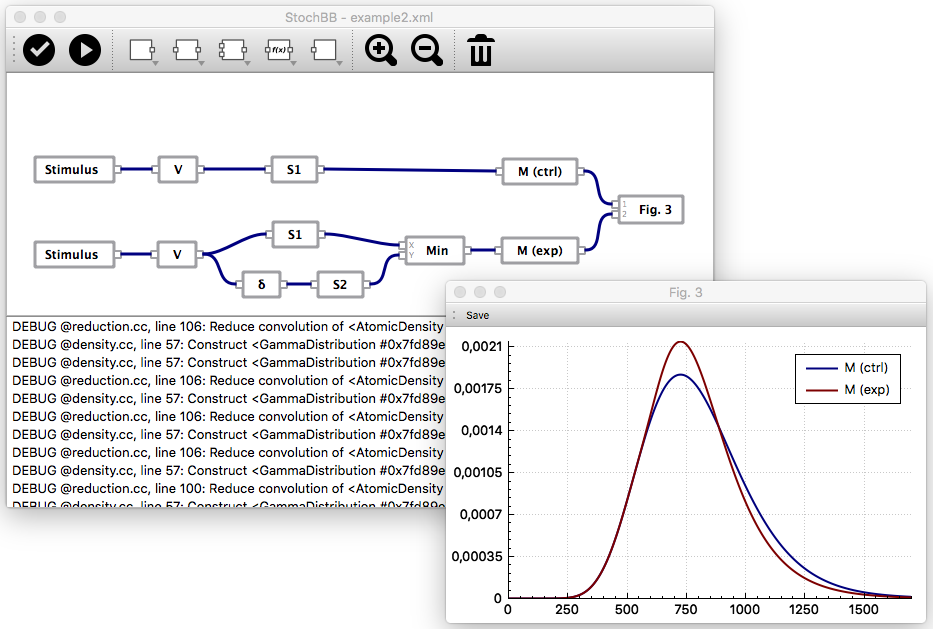
\includegraphics[width=.75\textwidth]{fig/GUI2.png}
 \caption{Overview of the GUI of \pkg{StochBB}, the toolbar at the top of the main window (background), main network edit field in the middle of the main window, the log view at the bottom of the main window (can be hidden) and a separate plot window at the foreground.} \label{fig:gui}
\end{figure}

\subsection{General overview}
The main window of the GUI (see Figure \ref{fig:gui}) consists of two main parts:
\begin{enumerate}
 \item The tool bar at the top of the main window. Here, frequently used actions are collected like verifying the network, performing the analysis,
 adding or removing items. All these actions are also available at the main menu (not shown in Fig. \ref{fig:gui}).
 \item The main network view at the center of the main window. Here the network of \emph{stages} can be viewed and edited. This view is described in more detail below.
\end{enumerate}

Additionally, there  is a log window at the bottom. By default, this view is hidden and can be enabled at the main menu under \emph{View} $\rightarrow$ \emph{Show log}. It displays various messages from the core library emitted during the verification and analysis of the network. 


\subsection{Editing a network}
Within the network view, the network is shown and can be assembled or modified. New items (e.g., stages) can be added to the network by selecting them from either the tool bar or from the menu under \emph{Edit} (see Figure \ref{fig:items} for some examples). These items can then be moved around in the network view by simply dragging them. An item can be removed by first selecting it with a single click and choosing \emph{Edit} $\rightarrow$ \emph{Remove} from the main menu or the \emph{Remove} button in the tool bar.

All network items have at least two properties that can be edited by double-clicking the item. Its label, shown inside the box representing the item in the network view, and a descriptive text (not shown) that allows to document the item. Many nodes, particularly those representing \emph{stages} with some parametric waiting-time distribution, have additional parameters that specify the waiting-time distribution. 

\begin{figure}[!ht]
 \begin{subfigure}[c]{0.2\textwidth}
   \centering
 	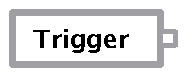
\includegraphics[width=0.8\textwidth]{fig/guitrigger.pdf}
 	\caption{Trigger/Stimulus item.} \label{fig:itemtrigger}
 \end{subfigure}\hfill
 \begin{subfigure}[c]{0.2\textwidth}
   \centering
 	
\includegraphics[width=0.45\textwidth]{fig/guigamma.pdf}
 	\caption{Gamma distr. random variable.} \label{fig:itemgamma}
 \end{subfigure}\hfill
 \begin{subfigure}[c]{0.2\textwidth}
   \centering
 	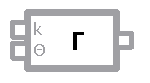
\includegraphics[width=0.65\textwidth]{fig/guigammac.pdf}
 	\caption{Compound Gamma distr. random variable.} \label{fig:itemgammac}
 \end{subfigure} \hfill
 \begin{subfigure}[c]{0.2\textwidth}
   \centering
 	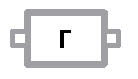
\includegraphics[width=0.6\textwidth]{fig/guigammap.pdf}
 	\caption{Gamma distr. stage.} \label{fig:itemgammap}
 \end{subfigure}
 
 \begin{subfigure}[c]{0.2\textwidth}
   \centering
 	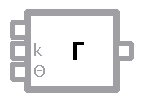
\includegraphics[width=0.6\textwidth]{fig/guigammacp.pdf}
 	\caption{Compound Gamma distr. stage.} \label{fig:itemgammacp}
 \end{subfigure}\hfill
 \begin{subfigure}[c]{0.2\textwidth}
   \centering
 	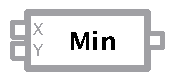
\includegraphics[width=0.8\textwidth]{fig/guimin.pdf}
 	\caption{Minimum stage.} \label{fig:itemmin}
 \end{subfigure}\hfill
 \begin{subfigure}[c]{0.45\textwidth}
   \centering
 	
\includegraphics[width=0.8\textwidth]{fig/guiinh.pdf}
 	\caption{Inhibition stage.} \label{fig:iteminh}
 \end{subfigure}
 
  \begin{subfigure}[c]{0.4\textwidth}
    \centering
 	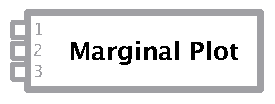
\includegraphics[width=0.6\textwidth]{fig/guiplot.pdf}
 	\caption{Marginal plot.} \label{fig:itemplot}
 \end{subfigure}\hfill
  \begin{subfigure}[c]{0.4\textwidth}
    \centering
 	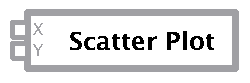
\includegraphics[width=0.55\textwidth]{fig/guiscatter.pdf}
 	\caption{Scatter plot.} \label{fig:itemscatter}
 \end{subfigure}
 \caption{Some examples of stages available in the GUI application.} \label{fig:items}
\end{figure}

All networks items have so-called sockets (small rectangles at the left or right side of the item, compare Fig. \ref{fig:items}). These sockets can be used to connect the items to form a network. All sockets on the left side of an item are input sockets and all on the right are outputs. Although a single output socket might be connected to several input sockets, every input can only be connected to single output socket. Like with network items, a connection can be removed by selecting it with a single click and choosing \emph{Edit} $\rightarrow$ \emph{Remove} from the main menu or the \emph{Remove} button in the tool bar.

All items can be divided into five groups: \emph{Random variables}, \emph{random stages}, \emph{join stages}, \emph{transformations} and \emph{plots}. \emph{Random variable} items (e.g., Figs. \ref{fig:itemtrigger}-\ref{fig:itemgammac}) represent simple random variables with some parametric distribution, which usually (except for compound random variables, e.g., Fig. \ref{fig:itemgammac}) have no input slots. One special item is the trigger or stimulus item (see Fig. \ref{fig:itemtrigger}). Although being a simple random variable with some $\delta$~distribution, that is a constant, it is mend to specify an event at a fixed time-point. There can be an arbitrary number of trigger items in every network (e.g. a stimulus at $T=0$ and a second manipulation of the experiment at some later time point).

All items of the \emph{random stage} group (e.g., Figs. \ref{fig:itemgammap}, \ref{fig:itemgammacp}) have a trigger input socket. Although being similar to the \emph{random variable} items, they might be considered as \emph{processing stages} with some parametric waiting-time distribution. That is, its output is a random variable being the sum of its input and a random variable distributed according to some parametric distribution. Like for the simple \emph{random variable} items, there are also \emph{random stage} items with a compound waiting-time distribution (e.g., Fig. \ref{fig:itemgammacp}).

As mentioned above, an input socket may only be connected to a single output socket, although a single output may be connected to several inputs. This is due to the fact, that the function for joining several \emph{signal paths} must be specified explicit. \emph{Join stages} (see Figs. \ref{fig:itemmin}, \ref{fig:iteminh}) are these functions that can be used to join signal paths according to some function. 

For example the \emph{minimum} stage (Fig. \ref{fig:itemmin}) represents the minimum of the inputs $X$ and $Y$. Or, in terms of processing stages, it gets triggered once either the stage connected to the $X$ input or the stage connected to the $Y$ input completed. A special \emph{join stage} is the \emph{inhibition} stage (Fig. \ref{fig:iteminh}). It represents the \emph{conditional sum} random variable introduced above and is the only stage represented by two items. The first item labeled \emph{inh} forwards the first event and inhibits the second. For example, it triggers only the stages connected to the $X$ output socket if the stage connected to the $X$ input completes first. The second item labeled \emph{join} then joins the two mutually exclusive signal paths into one. The \emph{conditional} random variable introduced above, is not included as a \emph{random stage} item as it would break causality.

Finally, the \emph{plot} items (see Figs. \ref{fig:itemplot}, \ref{fig:itemscatter}) allow for evaluating or sampling from the network. When added to the network, the \emph{Marginal Plot} item (Fig. \ref{fig:itemplot}) has no inputs at all. This item has a \emph{graphs} property that defines the number of graphs and consequently the number of inputs for this item. After this property has been set to the desired value, the corresponding number of inputs will appear at the item. In contrast, the \emph{Scatter Plot} item has always two inputs. They specify the two random variables to sample from for a scatter plot.

\subsection{Verifying the network and running an analysis}
Performing an analysis consists of two steps. In a first step, a network of random variables is derived from the stage-network representation used by the GUI application. This step will fail xif any assumption (e.g., independence assumptions) made by the derived random variables is not met. This step will fail too, if there is a cyclic dependency between stages or an unconnected input socket. Once the network of random variables is derived, it is ensured that the network is consistent. Hence running an analysis and verifying the network share this first step. 

In a second step, the derived network of random variables is actually analyzed. That is, the marginal distributions of the random variables being plotted are obtained and evaluated on the desired intervals. For the \emph{Scatter plots} or \emph{KDE plots}, a sampler gets instantiated to obtain samples from the random variables of interest. Finally, the plots are created and shown in separate plot windows.
\section{An example: The divergence point} \label{sec:pod}
This example shows a simple \emph{toy model} for some cognitive process that is able to produce a
so called \emph{divergence point} \cite[e.g.,][]{Reingold2012}. A divergence point of two response-latency
distributions is the earliest time point at which the two distributions differ. Obviously, 
there exists no divergence point, if the two distributions are analytic 
(e.g., the convolution of Gamma distributions, \cite{Mathai1982}) and there is some controversy
whether a cognitive model that is formed by simple \emph{processing stages} exists, which has a
divergence point \cite[e.g.,][]{Gomez2016}.

Within this example, I not only show how a non-analytic response-latency distribution may arise
using very common processing-stage models (i.e., these stages are also used in EZ-Reader model,
\cite{Reichle2003}) that allows for a divergence point, but actually has a divergence point%
\footnote{At least one distribution being non-analytic is a necessary but not a sufficient
condition for the existence of a divergence point.}. 

This very simple model consists of 4 Gamma-distributed stages $V, S_1, S_2$ and $M$,
where the second stage $S_2$ is delayed by $500$ ms. 
The model is
\begin{align}
 \text{control: } & R_c = V + S_1 + M \\
 \text{experimental: } & R_e = V + \min(S_1, 500+S_2) + M\,,
\end{align}
where $V \sim \Gamma(5,30),\,S_1\sim\Gamma(10,50)\,S_2\sim\Gamma(1,200)$ and $M\sim\Gamma(1,150)$.
\begin{figure}[!ht]
 \centering
 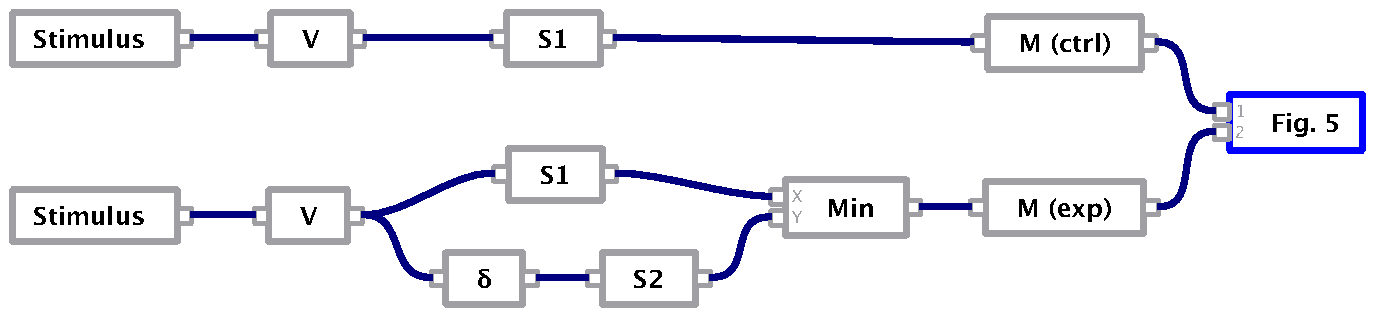
\includegraphics[width=0.9\textwidth]{fig/example2.pdf}
 \caption{Network of the second example model as visualized by \pkg{StochBB}.} \label{fig:example2}
\end{figure}

This model (also shown in Figure \ref{fig:example2}) can be read as: Under control condition, the
stimulus triggers a common \emph{visual} stage $V$ which then triggers a second stage $S_1$ that
itself immediately triggers the response stage $M$. Under experimental condition, again the
stimulus triggers the common stage $V$ which then triggers $S_1$. Additionally to the stage $S_1$,
$V$ also triggers the delayed stage $S_2$ in parallel to $S_1$. The response stage $M$ is then triggered by 
either $S_1$ or $S_2$, depending on which stage completes first. Consequently, the response latency
under experimental condition is $R_e = V + \min(S_1,S_2+500) + M$.

\begin{figure} [!ht]
 \begin{subfigure}[t]{0.45\textwidth}
   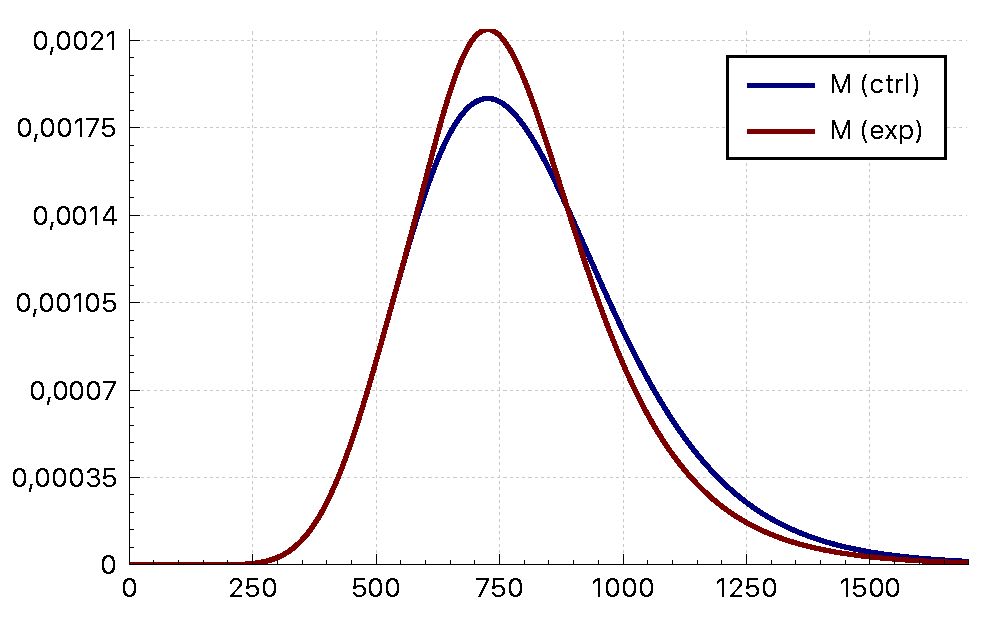
\includegraphics[width=.95\textwidth]{fig/example2_plot.pdf}
   \subcaption{PDFs of the response latencies under control condition (blue lines) and experimental condition (red lines).  
   The \emph{true} divergence point of the two response-latency distributions is $500$ ms, however, the distributions appear 
   to diverge much later (about $600$ ms). \label{fig:pod}}
  \end{subfigure} \hfill
 \begin{subfigure}[t]{0.45\textwidth}
   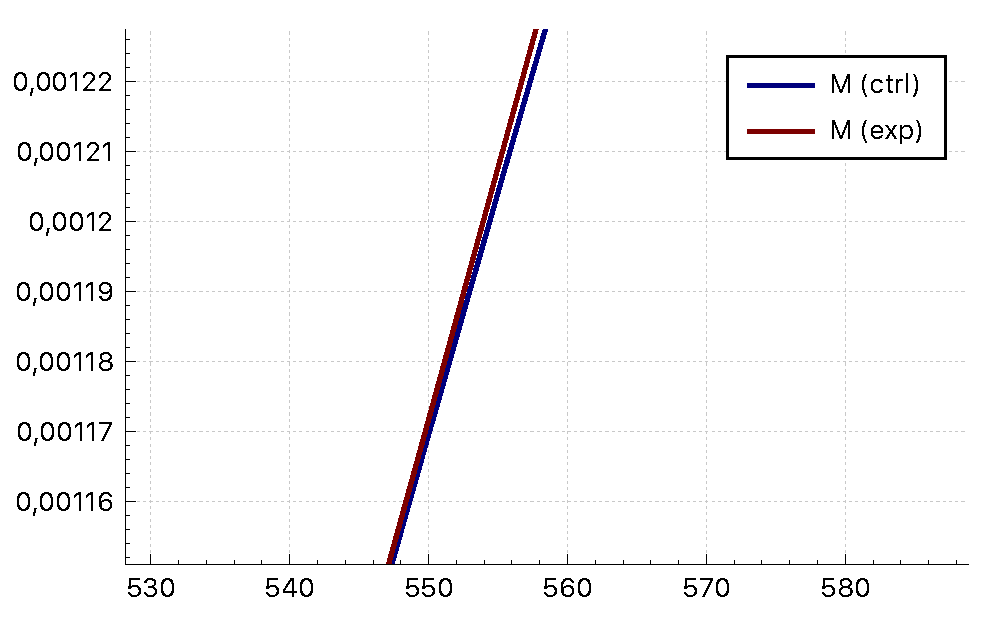
\includegraphics[width=.95\textwidth]{fig/example2_zoom_plot.pdf}
   \subcaption{The same PDFs but zoomed in. Here it get visible that the \emph{true} PD is much earlier that visible in the right plot. In fact the \emph{true} DP is not visible under any zoom level, as the PDFs diverge very slowly.} \label{fig:podzoom}
  \end{subfigure}
  \caption{Comparison of the response latency distributions as obtained from the mode shown in Fig. \ref{fig:example2}.}
  \label{fig:podplots}
\end{figure}

Figure \ref{fig:podplots} shows the plots generated by \pkg{StochBB}. The blue lines show the PDF
of the response latency under control condition. Being a convolution of 3 Gamma distributions, it 
is an analytic function on the interval $(0,\infty)$ \citep{Mathai1982}. The red lines show the 
PDF of the response latency under experimental condition. As the distribution of $S_2$ is not analytic on 
the complete interval $(0,\infty)$ (discontinuity at $T=500$ ms), a divergence point may exist at 
$T=500$. 

Due to the \emph{minimum} stage and the fact that $P(S_2<500)=0$ (delayed by 
$500$ ms), it is ensured that the two response latencies are identical on the interval $[0,500)$ ms.
Hence, this simple model is able to produce a divergence point as both response-latency distributions are identical
on the interval $[0,500)$ and diverge thereafter.

However, Fig. \ref{fig:podzoom} shows that this divergence point cannot be estimated reliably from
a finite data set as the two response latency distributions diverge very slowly%
\footnote{In fact, the distribution of the response latency under experimental condition is an
example of a $C^\infty$-function, that is a smooth function, that is not analytic
($\notin C^\omega$).}. Consequently, an estimate for this point \cite[e.g. by means of estimators 
proposed in][]{Reingold2012} based on a finite sample will always be heavily biased towards larger
values. Moreover, if the experimental manipulation also affects the parameters of the $V, S1$ or 
$M$ stage, the two response distributions will be different everywhere on the interval
$(0,\infty)$ and consequently no divergence point exists. For a finite data set, however, an
estimator \cite[like][]{Reingold2012} will always report a finite estimate as it is simply impossible
to test for the existence of a divergence point on a finite data set. 
\section{Dealing with data} \label{sec:data}
Given that \pkg{StochBB} is able to provide good approximations for the marginal PDFs of some
(response) random variable, it is also able to fit a system of dependent random variables to data.
For this, the \pkg{StochBB} API provides two functions. One is the \code{kolmogorov} function
which returns the Kolmogorov-Smirnov statistic \cite[KS-statistic, e.g.,][]{Kolmogorov1933,
Smirnov1948, Marsaglia2003}, the other function is the \code{logLikelihood} function. Both take
the random variable, the number of bins and some data vector as arguments. These functions then
uses an approximation of the PDF (for the log likelihood) or CDF (KS-statistic) evaluated on a
regular grid spanning at least the data range for computing the corresponding value.

They can then be used to fit a network of random variables to some given observations. For
example, consider the network of random variables introduced in the divergence point example 
above, describing the cognitive
process under the \emph{experimental condition}. One may try to re-estimate the $\theta=120$
parameter of the stage S2. First, a relatively large sample is drawn ($N=30,000$). Then one may
implement a cost function of that parameter. Here, the negative of the log likelihood, given the
samples is used. Finally the model is fitted to the the data by minimizing the cost function using
a numerical optimization algorithm.

An example R code could be
\begin{lstlisting}[language=R, basicstyle=\footnotesize]
library(stochbb)

# The "stages"
d  <- 500
V  <- gamma(5,30)
S1 <- gamma(10,50)
S2 <- gamma(1,120)
M  <- gamma(1,150) 

# Response under "experimental condition"
Re <- V %+% minimum(S1, S2 %+% d) %+% M

# Sample Re
Nsam <- 30000;
sam <- new(ExactSampler, c(Re))
res <- array(0, c(Nsam,1))
sam$sample(res)

costFunc <- function(theta) {
  S2 <- gamma(1,theta[1]);
  R <- V %+% minimum(S1, affine(S2, 1, d)) %+% M
  return( -logLikelihood(R, 10000, res[,1]) )
}

# Find estimate
opt <- optim(c(100), costFunc, method="L-BFGS-B")
\end{lstlisting}

This code is then able to find the $\theta$ parameter for the S2 stage by means of maximum likelihood (see Figure
\ref{fig:llprof}). 

\begin{figure}[!ht]
 \centering
 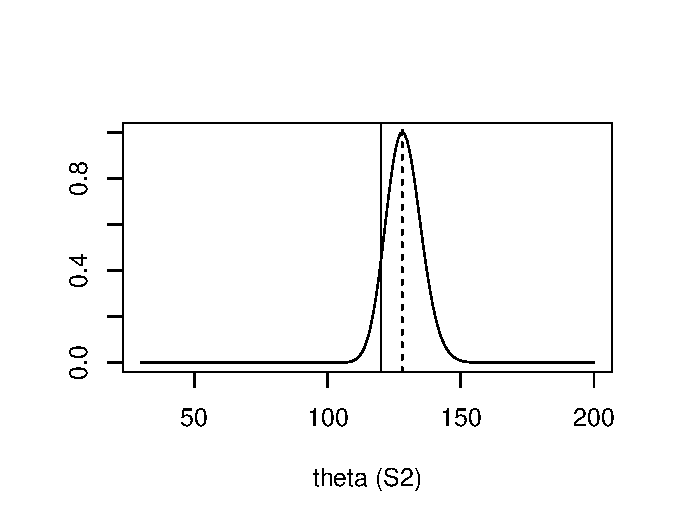
\includegraphics[width=0.49\textwidth]{fig/pod_likelihoodProf.pdf}
 \caption{An example of a likelihood profile for some $\theta$ estimate (vertival dashed line)
 using 30,000 samples drawn from a network of random variables, with $\theta=120$ (vertical
 solid line) for the $S1$ stage.} \label{fig:llprof}
\end{figure}

Moreover, the \code{logLikelihood} can then also be used to profile the likelihood (compare Figure
\ref{fig:llprof}) given the data to obtain confidence intervals for the parameter estimate. There
the true value of $\theta=120$ is shown as a solid vertical line and the estimate as the dashed
vertical line. 	
\section{Summary}
\begin{itemize}
 \item \pkg{StochBB} allows to analyze systems of dependent random variables efficiently without resorting to stochastic simulation.
 \item It uses analytic solutions for the marginal distributions if possible and resorts to numerical approximations if necessary.
 \item To this end, it reveals a surprising good precision. One that would require a large amount of samples to achieve same precision using stochastic simulation.
 \item The GUI eases the assembly of complex networks that are mend to describe random models like those typical for cognitive psychology.
 \item The software (including the core library, interfaces to \proglang{Python} and \proglang{R} as well as the graphical user interface) is available under the General Public License version 3 at \texttt{https://github.com/stochbb}. 
\end{itemize}

\bibliography{references}

\appendix
\section{Application programming interface} \label{sec:api}
The application programming interface \cite[API, see also][]{stochbbapi} 
allows to assemble complex systems of random variables programmatically in C++.
All API classes are derived from the \code{Container} class which is an essential part of the
memory management system used by \pkg{StochBB}. Usually a C++ programmer needs to keep track of all
objects still in use and is responsible to free unneeded objects to avoid memory leaks. This can
be a difficult task when dealing with complex structured objects cross-referencing each other.
To ease the usage of \pkg{StochBB}, a \emph{mark and sweep} garbage collector is implemented which keeps track
of all objects being directly or indirectly reachable and freeing all unreachable objects. For
this memory management system to work, it is necessary to treat all container objects like values
although they represent references to objects allocated on the heap.

There are also Python and R packages (called \code{stochbb} too) that provide access to
the classes and functions of the C++ API. This allows for a convenient construction of systems
of random variables while maintaining the speed of the C++ implementation. These APIs are 
almost identical to the C++ one that R and \code{numpy} array are used instead of Eigen matrices
and vectors.

The central class of \pkg{StochBB} is \code{Var}, representing a random variable. This could be a
simple random variable having a specified distribution (\code{AtomicVar}) or a random
variable that is derived from others like \code{Chain}, \code{Minimum}, \code{Maximum} or
\code{Mixture}. All random variables (atomic and derived) have probability density functions
attached. They can be accessed using the \code{Var::density} method which returns a 
\code{Density} object.

All \code{Density} objects have two methods, \code{Density::eval} evaluating the probability
density function and \code{Density::evalCDF} evaluating the cumulative density or probability
function. Assembling a system of random variables and evaluate their PDFs or CDFs is straight
forward. Sampling, however, is not that trivial and is described below in some detail.

\subsection{Assembling a system of random variables}
In a first step, one may define a new gamma-distributed random variable with shape $k=10$
and scale $\theta=100$ as
\begin{lstlisting}[language=C++]
 #include <stochbb/api.h>
 using namespace stochbb;
 
 // [...]
 
 Var X1 = gamma(10, 100);
\end{lstlisting}

Its PDF can then be evaluated as on a regular grid in $[0,1000)$ with $1000$ grid points as
\begin{lstlisting}[language=C++]
 // [...]
 
 Eigen::VectorXd pdf(1000);
 X1.density().eval(0, 1000, pdf);
\end{lstlisting}

The result of the evaluation is stored into the vector \code{pdf}. There are only very few basic
or atomic random-variable types defined in \pkg{StochBB}:

\begin{tabular}{l|lp{8.4cm}l}
 Constructor & Parameters & Process description \\ \hline
 \code{stochbb::delta} & \code{delay} & A constant delay or a process with a fixed waiting time. \\
 \code{stochbb::unif} & \code{a}, \code{b} & A process with a uniform-distributed waiting time. \\
 \code{stochbb::norm} & \code{mu}, \code{sigma} & A process with a normal-distributed \emph{waiting time}. \\
 \code{stochbb::gamma} & \code{k}, \code{theta} & A process with a gamma-distributed waiting time. \\
 \code{stochbb::invgamma} & \code{alpha}, \code{beta} & A process with an inverse gamma-distributed waiting time. \\
 \code{stochbb::weibull} & \code{k}, \code{lambda} & A process with a Weibull-distributed waiting time. \\
 \code{stochbb::studt} & \code{nu} & A process with a Student's t-distributed \emph{waiting time}. \\
\end{tabular}

More complex processes can be derived by combining these atomic random variables or as special cases of them. 
For example, the exponential distribution $\text{Exp}(\lambda)$ is equivalent to a Gamma distribution with $k=1$ 
and $\theta = \lambda^{-1}$.

\subsubsection{Affine transformation of random variables}
An affine transformation of a random variable $X$ is of the form $a\,X+b$, where $a\neq 0$ and $b$ are
real values. An affine transformation can be obtained using the overloaded * and + operators or using the
\code{stochbb::affine} function. For example, the code
\begin{lstlisting}[language=C++]
 #include <stochbb/api.h>
 using namespace stochbb;
 
 // [...]
 
 Var X = gamma(10, 100);
 Var Y = 3*X + 1;
\end{lstlisting}
constructs a random variable \code{Y} being an affine transformed of the random variable \code{X}.

\subsubsection{Sums of random variables}
Beside the affine transfrom of random variables, the most basic derived random variable is a \code{Chain}.
This type represents the \emph{chaining} of random processes. Such a chain can be constructed using 
the overloaded \code{+} operator or the \code{stochbb::chain} function. For example
\begin{lstlisting}[language=C++]
 #include <stochbb/api.hh>
 using namespace stochbb;

 // [...]

 Var X1 = gamma(10,100);
 Var X2 = gamma(20, 50);
 Var Y = X1 + X2;
\end{lstlisting}

\subsubsection{Minimum and Maximum of random variables}
Another simple derived random variable is the \code{Maximum} or \code{Minimum} class. As the
names suggest, they represent the maximum or minimum of a set of random variables. They can be
created using the overloaded standard library function \code{std::min} and \code{std::max} or the
\code{stochbb::minimum} and \code{stochbb::maximum} functions. The latter take a vector of random variables.
\begin{lstlisting}[language=C++]
 #include <stochbb/api.hh>
 using namespace stochbb;

 // [...]

 Var X1 = gamma(10, 100);
 Var X2 = gamma(20, 50);
 Var Y = std::max(X1, X2);
\end{lstlisting}

\subsubsection{Conditional random variables}
Conditional random variables as described above, can be created using the 
function \code{stochbb::\allowbreak cond} as following. 
\begin{lstlisting}[language=C++]
 #include <stochbb/api.hh>
 using namespace stochbb;

 // [...]

 Var X1 = gamma(10, 100);
 Var X2 = gamma(20, 50);
 Var Y1 = normal(0, 1)
 Var Y2 = normal(0, 2);
 Var Z = cond(X1,X2, Y1,Y2);
\end{lstlisting}

\subsubsection{Conditional sums of random variables}
Likewise the simple conditional random variable, conditional sums of random variables can be constructed 
using the \code{stochbb::\allowbreak condsum} function as 
\begin{lstlisting}[language=C++]
 #include <stochbb/api.hh>
 using namespace stochbb;

 // [...]

 Var X1 = gamma(10, 100);
 Var X2 = gamma(20, 50);
 Var Y1 = normal(0, 1)
 Var Y2 = normal(0, 2);
 Var Z = condsum(X1,X2, Y1,Y2);
\end{lstlisting}

\subsubsection{Mixtures of random variables}
Similar to the \code{Minimum} or \code{Maximum}, a mixture of random variables can be
constructed using the \code{stochbb::mixture} function. This function takes a at least 
two variables and their associated weight. Such a mixture can be considered as a random process which
randomly selects the outcome of a set of other random processes, where the probability of
selecting a specific process is given by the relative weight assigned to each process.
\begin{lstlisting}[language=C++]
 #include <stochbb/api.hh>
 using namespace stochbb;

 // [...]

 Var X1 = gamma(10,100);
 Var X2 = gamma(20, 50);
 Var Y = mixture(1,X1, 2,X2);
\end{lstlisting}

In the example above, the random process $Y$ will select the outcome of $X_1$ with
a probability of $\frac{1}{3}$ and the outcome of $X_2$ with probability
$\frac{2}{3}$.

\subsubsection{Compound random variables}
An important class of derived random processes are compound processes. There the parameters of the
distribution of a random variable are themselves random variables. That is
\begin{equation}
 X \sim f(x|A)\,,\quad A \sim g(a|\theta)\,, \nonumber
\end{equation}
where the random variable $X$ is distributed as $f(x|A)$, parametrized by $A$,
where $A$ itself is a random variable distributed as $g(a|\theta)$, parametrized by
$\theta$. 

Compound random variables are created using the same factory function like the atomic random variable
types. In contrast to the atomic random variables, the factory functions take random variables as 
parameters instead of constant values.
\begin{lstlisting}[language=C++]
 #include <stochbb/api.hh>
 using namespace stochbb;
 
 // [...]
 
 Var mu = gamma(10,100);
 Var cnorm = norm(mu, 10);
\end{lstlisting}
instantiates a compound-normal distributed random variable, where the mean is gamma distributed
while the standard deviation is fixed.

\subsection{Sampling several dependent random variables}
As mentioned above, sampling efficiently from a complex system of random variables is not trivial. 
First of all, it must be ensured that all atomic random variables are sampled only once. Otherwise, two dependent
random variables may be sampled as independent. Moreover, the samples of derived random variables
should be cached for efficiency. 

\pkg{StochBB} provides a separate class that implements a proper sampler for a system
of random variables, the \code{ExactSampler} class. This class allows to sample
from several possibly dependent random variables simultaneously. Upon construction,
the set of random variables to sample from, is specified. A sample from these random
variables can then be obtained by the \code{ExactSampler::sample} method.
\begin{lstlisting}[language=C++]
 #include <stochbb/api.hh>
 using namespace stochbb;

 // [...]

 Var X1 = gamma(10,100);
 Var X2 = gamma(20, 50);
 Var Y = std::min(X1, X2);
 // Construct sampler
 ExactSampler sampler(X1, X2, Y);
 // Get 1000 samples
 Eigen::MatrixXd samples(3, 1000);
 sampler.sample(samples);
\end{lstlisting}

The \code{ExactSampler::sample} method takes a reference to a \code{Eigen::Matrix} where each column
represents the random variable given to the constructor and each row an independent sample from
the system.

For very large systems, sampling may get slow. Particularly if one is only interested
in the marginal distribution of single random variables. For these cases, an approximate sampler
for single random variables is provided, the \code{MarginalSampler}. This sampler uses an
approximation of the inverse of the cumulative distribution function of a random variable
to draw samples.
\begin{lstlisting}[language=C++]
 #include <stochbb/api.hh>
 using namespace stochbb;

 // [...]

 Var X1 = gamma(10,100);
 Var X2 = gamma(20, 50);
 Var Y = std::min(X1, X2);
 // Sample from Y on [0,500] in 1000 steps
 MarginalSampler sampler(Y, 0, 500, 1000);
 // Get 1000 samples
 Eigen::VectorXd samples(1000);
 sampler.sample(samples);
\end{lstlisting}

In this example, a \code{Marginal\-Sampler} is constructed for the random variable \code{Y}. Using an
approximation of its CDF on the interval $[0,500)$ using $1000$ steps. Then, the
\code{Marginal\-Sampler::\allowbreak sample} method is used to obtain $1000$ independent samples.

\subsection{Handling data}
Being able to evaluate the CDFs and PDFs of random variables efficiently, \pkg{StochBB} can be
used to fit a system of random variables to observations by either maximizing the (log) likelihood
or minimizing the Kolmogorov-Smirnov statistic \cite[KS; e.g.,][]{Marsaglia2003}. For these tasks,
\pkg{StochBB} provides two functions. One called \code{kolmogorov}, evaluating the KS statistic
and the other is called \code{logLikelihood} evaluating the log likelihood of some given data for
a specific random variable. Both functions share the same interface (continuing the example above)

\begin{lstlisting}[language=C++]
// [...]

// evaluate the KS statistic of the data samples for RV Y
kolmogorov(Y, 0, 500, 1000, samples);
// or evaluate the log likelihood
logLikelihood(Y, 0, 500, 1000, samples);
\end{lstlisting}

The first argument specifies the random variable, here \code{Y}. the next two arguments specify
the range on which the CDF or PDF is evaluated, here $[0,500)$. The fourth argument specifies the
number of bins to use for the evaluation (here $1000$) and finally the fifth argument specifies
the data vector. Please note that both functions may log a warning message if some given samples
lay outside of the specified interval. Both functions will then simply ignore these values.

\end{document}
